% ЕМТ 2025, VIII клас — точен LaTeX препис от официалните файлове в Klasirane.com.
% Условия: https://klasirane.com/api/competitions/EMT/All/2025/8%20%D0%BA%D0%BB/probs
% SHA-256 (условия): 0cbce19283d213ccc369f9c674573d5fa725e95a9d72288e147f331039984c27
% Решения: https://klasirane.com/api/competitions/EMT/All/2025/8%20%D0%BA%D0%BB/sol
% SHA-256 (решения): 4db51c345b543b908d5a731a153107dd962838cfc3549a230b6f10fdcca8157e
% Точковите оценки, правописът и формулировките са запазени от източника.
% Файлът с условията е едностранично сканирано изображение; видимата страница е проверена пряко.

Задача 8.1. Числата $a,b,c,x$ изпълняват равенствата

$$x^2-a+1=x^3-b=x^4-c+1\quad\text{и}\quad(a-b)^2+3=2(a+c-2b).$$

Да се намерят всички възможни стойности на $x$.

Отговор. $-1,0,1,2$

Решение. (Първи начин) Имаме $b-a=x^3-x^2-1$ и $c-b=x^4-x^3+1$. Заместване в

$$(b-a)^2+3=2((c-b)-(b-a))$$

води до еквивалентното

$$(x^3-x^2-1)^2+3=2(x^4-2x^3+x^2+2).$$

След разкриване на скобите и съкращаване се получава $x^6-2x^5-x^4+2x^3=0$, което се разлага до

$$x^3(x-1)(x+1)(x-2)=0.$$

Следователно $x$ може да бъде само $-1,0,1,2$. (За всяко такова $x$ възможните $a,b,c$ се определят изцяло от $b-a=x^3-x^2-1$ и $c-b=x^4-x^3+1$.)

(Втори начин) Имаме $a-b-1=x^2-x^3$ и $c-b-1=x^4-x^3$. Равенството $(a-b)^2+3=2(a+c-2b)$ е еквивалентно на $(a-b-1)^2=2(c-b-1)$. Оттук

$$2x^3(x-1)=x^4(x-1)^2,$$

което се разлага до

$$x^3(x-1)(x+1)(x-2)=0.$$

Следователно $x$ може да бъде само $-1,0,1,2$. (За всяко такова $x$ възможните $a,b,c$ се определят изцяло от $b-a=x^3-x^2-1$ и $c-b=x^4-x^3+1$.)

Оценяване. (6 точки) 3 т. за достигане на уравнение само на променливата $x$ (от които 1 т. за изразяване на $b-a$ чрез $x$, 1 т. за изразяване на $c-b$ чрез $x$ и 1 т. за заместване в даденото равенство за $a,b,c$), 2 т. за получаване на разложен вид само с линейни множители (от които 1 т. ако е достигнато до уравнение от най-много трета степен в нормален вид при разкрити скоби), 1 т. за окончателен отговор.

Задача 8.2. Даден е успоредник $ABCD$. Ъглополовящите на ъглите $\angle DAC$ и $\angle DBC$ се пресичат в точка $K$. Известно е, че:

• Разстоянието от $K$ до правата $AD$ е равно на разстоянието от $K$ до правата $BC$.

• Разстоянието от $K$ до правата $AB$ е девет пъти по-дълго от разстоянието от $K$ до правата $CD$.

Да се намери отношението $AB:AD$.

Отговор. $3:4$

Решение. Нека $AC\cap BD=O$. Имаме

$$OK\parallel AD\parallel BC,$$

понеже $K$ и $O$ са на равни разстояния от $AD$ и $BC$ (за $K$ – по условие, за $O$ – от $\triangle AOD\cong\triangle BOC$).

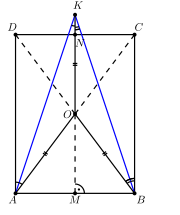
\includegraphics[max width=0.34\textwidth, alt={Правоъгълникът ABCD и точките K, O, M и N от официалното решение}, center]{assets/8-2-rectangle.svg}

Оттук $\angle AKO=\angle KAD=\angle KAO$, съответно $AO=OK$. Аналогично $BO=OK$, следователно $AO=BO$, т.е. $AC=BD$, оттук $ABCD$ е правоъгълник.

Понеже $ABCD$ е правоъгълник и $K$ и $O$ са на равни разстояния от $AD$ и $BC$, то $K$ и $O$ лежат на общата симетрала $MN$ на $AB$ и $CD$, където $M$ и $N$ са средите на $AB$ и $CD$. Освен това, от $OK=AO>OM=ON$ следва, че $N$ е между $K$ и $O$.

При $KN=x$ от даденото имаме $MK=9x$, оттук

$$MO=ON=\dfrac{MK-NK}{2}=4x.$$

Така $AO=OK=ON+NK=5x$ и $AM=\sqrt{AO^2-OM^2}=3x$ от Питагоровата теорема за $\triangle AOM$. Окончателно $AB=2AM=6x$, $AD=MN=8x$ и $AB:AD=3:4$.

Оценяване. (6 точки) 1 т. за доказване на някое от $AO=OK$ и $BO=OK$, 1 т. за доказване, че $ABCD$ е правоъгълник, 1 т. за получаване на $MO=ON=4KN$, 1 т. за получаване на $AO=5KN$, 1 т. за получаване на $AM=3KN$, 1 т. за окончателен отговор.

Задача 8.3. Ивайло избрал няколко различни (краен брой, поне две) прости числа с произведение $n$, като за всяко избрано просто число $p$ е изпълнено, че $4n$ се дели на $p^2-1$. Да се намерят всички възможни стойности на $n$.

Отговор. $6,30,330$

Решение. Нека $p_1<p_2<\cdots<p_k$, $k\ge2$, са избраните прости числа. Не е възможно всичките да са нечетни, понеже тогава $4n$ не се дели на 8, докато $p^2-1=(p-1)(p+1)$ се дели на 8 за всяко нечетно $p$. Оттук $p_1=2$. Сега получаваме, че $2^2-1=3$ е делител на $4n$, съответно $p_2=3$. Ако $k=2$, то $n=p_1p_2=6$; нека $k\ge3$.

Да отбележим, че ако $j\ge i\ge3$, то $\operatorname{НОД}(p_i-1,p_j)=\operatorname{НОД}(p_i+1,p_j)=1$, тъй като $p_j$ е просто и надвишава $p_i-1$, а не дели и $p_i+1$ понеже надвишава $\dfrac{p_i+1}{2}$ при $p_i\ge5$, докато $p_j=p_i+1$ е невъзможно поради четност. Така непременно $p_3^2-1$ дели $4\cdot2\cdot3=24$ и с $p_3\ge5$ получаваме само $p_3=5$. Ако $k=3$, то $n=30$; нека $k\ge4$.

Непременно $p_4^2-1$ дели 120 и предвид $p_4>p_3=5$ получаваме само $p_4=11$, тъй като $7^2-1=48$ не дели 120. Ако $k=4$, то $n=330$; нека $k\ge5$.

Необходимо е $p_5^2-1$ да дели 1320, еквивалентно на $\dfrac{p_5^2-1}{8}$ да дели 165. Предвид $p_5>p_4=11$ и $8\cdot15+1=11^2$, работим само с делителите на 165, по-големи от 15, които са 165, 55, 33. Обаче $165\cdot8+1=1321\in(36^2,37^2)$ и $33\cdot8+1=265=5\cdot53$ не са точни квадрати, а $55\cdot8+1=21^2$ би дало $p_5=21$, което не е просто число. Окончателно $k\ge5$ е невъзможно.

Оценяване. (7 точки) 1 т. за доказване на $p_1=2$, 1 т. за доказване на $p_2=3$, 1 т. за доказване на $p_3=5$, 1 т. за доказване на $p_4=11$, 2 т. за отхвърляне на $k\ge5$, 1 т. за напълно верен отговор.

Задача 8.4. (7 точки) Дадени са 15 точки, разположени на равни разстояния по окръжност. Всеки две от точките са свързани с отсечка.

Пътека ще наричаме редица от две по две различни отсечки, такива че всяка, освен първата, има общ край с предишната и никои три последователни отсечки в редицата нямат общ край. Колко най-много отсечки може да има по пътека, ако никои две от тях не лежат на две прави, сключващи ъгъл $60^\circ$?

На фигурата е показана пътека, съставена от седем отсечки.

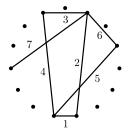
\includegraphics[max width=0.27\textwidth, alt={Пътека от седем отсечки между 15 равноотдалечени точки}, center]{assets/8-4-example.svg}

Отговор. 31

Решение. Да означим точките с $A_1,A_2,A_3,\ldots,A_{3n}$, където $n$ е нечетно число (тук $n=5$). Общият брой отсечки е $\dfrac{3n(3n-1)}{2}$, съответно отсечките могат да се разбият на $3n$ групи от по $\dfrac{3n-1}{2}$ взаимно успоредни отсечки. Да номерираме групите с $1,2,3,\ldots,3n$, като в група $i$ са успоредните на $A_iA_{i+1}$ (считаме $A_{3n+1}=A_1$). Тъй като $60^\circ=\dfrac{1}{3}\cdot180^\circ$, то две отсечки сключват ъгъл $60^\circ$ тогава и само тогава когато принадлежат на две различни групи с номера, които дават един и същи остатък при деление на $n$.

Да разгледаме всички отсечки от произволни $n$ групи с номера, които дават различни остатъци при деление на $n$. Нека от точките излизат съответно $k_1,k_2,\ldots,k_{3n}$ на брой от избраните отсечки. Във всяка пътека има не повече от две точки, от които излизат нечетен брой отсечки, тъй като нечетен брой може да има евентуално само при двата края на пътеката. Тъй като $k_i\le n$ (понеже групите са $n$ на брой) и $n$ е нечетно число, то от $3n-2$ от точките излизат не повече от $n-1$ (четно число) от избраните отсечки. Следователно

$$\sum_{i=1}^{3n}k_i\le(3n-2)(n-1)+2n=3n^2-3n+2.$$

Оттук получаваме, че броят на отсечките по пътека с желаното свойство не надвишава

$$\dfrac{3n^2-3n+2}{2},$$

тъй като всяка отсечка е броена по два пъти в горната сума.

За пример с $\dfrac{3n^2-3n+2}{2}$ отсечки можем да изберем всички отсечки от групите с номера $1,2,3,\ldots,n$ и да изключим $n-1$ от отсечките в група с номер $s=\dfrac{n+1}{2}$, които са най-близо до отсечката $A_sA_{s+1}$. При $n=5$ този брой е 31, като на фигурата възможна пътека започва от $A_8$ и завършва в $A_{14}$.

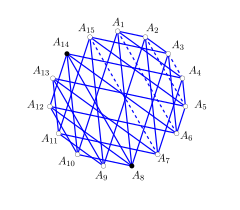
\includegraphics[max width=0.46\textwidth, alt={Официалната конструкция на пътека с 31 отсечки}, center]{assets/8-4-construction.svg}

Оценяване. (7 точки) 1 т. за получаване, че по пътеката няма две отсечки от групи с еднакъв остатък при деление на 5, 2 т. за получаване, че при 5 групи с различни остатъци при деление на 5 е изпълнено, че 5 точки са краища на 4 отсечки и 10 точки са краища на 5 отсечки, 1 т. за пресмятане на общия брой от 35 отсечки в петте групи, 1 т. за елиминиране на 4 от отсечките поради нечетност, 2 т. за работещ пример с 31 отсечки.
